\section{Amplitude Formalism}
{\color{red}TODO: cite http://scipp.ucsc.edu/\textasciitilde haber/ph218/ExperimentersGuideToTheHelicityFormalism.pdf and S.U. Chung spin formalisms}

Now we embark on the topic of amplitudes. We wish to describe the dynamics of our reaction in a way that allows us to extract quantum numbers like spin from our data. There are several difficulties in doing so: First, we are trying to determine the properties of many particles at once, and we know that many resonances in this channel overlap in mass space. This precludes the use of a simple Breit-Wigner description of most of these resonances, as overlapping Breit-Wigners do not preserve unitarity{\color{red}TODO: citation}. Second, the GlueX experiment uses a linearly polarized photon beam, so it behooves us to use a formalism which can include this polarization. Finally, there are many resonances in this channel, and while we have the largest photoproduction dataset to date, we are still relatively data limited, which further complicates any dynamical description.

\subsection{Single-Particle Helicity States}

We begin by defining a set of observables which are independent of frames and rotations on those frames. This is known as the helicity formalism, where helicity resembles the spin projection along the axis of a particle's motion. First, we define a rotation $R(\alpha, \omega, \gamma)$ as a matrix whose action on a vector is a rotation about the Euler angles $\alpha$, $\omega$, and $\gamma$. For each rotation, we can define a unitary operator $U[R]$ which has the group property $U[R_2 R_1] = U[R_2] U[R_1]$ as it is an operator on the group $SO(3)$. Being an operator on $SO(3)$, we can also write it as

\begin{equation}
  U[R(\alpha,\omega,\gamma)] = e^{-\imath \alpha J_z} e^{-\imath \omega J_y} e^{-\imath \gamma J_z}
  \label{eq:rotation-rep}
\end{equation}

We can then describe the matrix elements of this operator in the angular momentum eigenbasis $\ket{jm}$ (representing a spin-$j$ particle where $m$ is the projection of spin onto the $\hat{z}$-axis) with the Wigner D-matrix:

\begin{gather}
  U[R(\alpha, \omega, \gamma)] \equiv \sum_{m'} \ket{jm} D_{m'm}^j(R(\alpha, \omega, \gamma)) \\
  \text{where} \notag\\
  D_{m'm}^j(\alpha, \omega, \gamma) \equiv e^{-\imath m' \alpha} d_{m'm}^j e^{-\imath m\gamma} \\
  \text{and} \notag\\
  d_{m'm}^j(\omega) = \mel{jm'}{e^{-\imath\omega J_y}}{jm}
  \label{eq:wigner-d-definition}
\end{gather}

We can further extend this eigenbasis to include linear momentum by introducing Lorentz boosts $L(\vec{\beta})$. We denote the operation of a boost along the $\hat{z}$-axis with velocity $\beta$ as $L_z(\beta)$. A boost in any direction described by polar angles $(\theta, \varphi)$ can be achieved by rotating the $\hat{z}$-axis to align with the direction vector, boosting in the new $\hat{z}$-direction, and rotating back:

\begin{equation}
  L(\vec{\beta}) = R(\varphi, \theta, 0) L_z(\beta) R^{-1}(\varphi,\theta,0)
\end{equation}

Together, the space of rotations and boosts defines the Lorentz group, where each arbitrary Lorentz transformation $\Lambda$ has a unitary operator $U[\Lambda]$ with the group property $U[\Lambda_2 \Lambda_1] = U[\Lambda_2]U[\Lambda_1]$, so in terms of operators, we can also write

\begin{equation}
  U[L(\vec{p})] = U[R(\varphi, \theta, 0)]U[L_z(p)]U^{-1}[R(\varphi,\theta,0)]
\end{equation}

Finally, this allows us to define the ``canonical'' basis for a single particle as
\begin{equation}
  U[L(\vec{p})]\ket{jm} \equiv \ket{\vec{p},jm}
  \label{eq:canonical-single-particle}
\end{equation}

Unfortunately, the quantum number $m$ is only valid in the rest frame of the state because the $\hat{z}$-axis of the rest frame is not equivalent to the $\hat{z}$-axis in any arbitrarily Lorentz-transformed frame. Therefore, we will define helicity $\lambda$ as the projection of spin along the direction of motion and introduce new helicity states,

\begin{equation}
  \ket{\vec{p},j\lambda} = U[L(\vec{p})]U[R(\varphi,\theta,0)]\ket{j\lambda} = U[R(\varphi,\theta,0)]U[L_z(p)]\ket{j\lambda}
  \label{eq:helicity-single-particle}
\end{equation}

In this definition, we have two ways of obtaining the helicity frame: We can either rotate the state first such that the quantization axis is aligned with $\vec{p}$ and then boost in the $\hat{p}$-direction or we can first boost in the $\hat{z}$-direction and then rotate. In either equivalent case, $\lambda$ is invariant under rotations as well as boosts parallel to $\vec{p}$. Finally, we can define these helicity states over a basis of canonical states:

\begin{equation}
  \ket{\vec{p},j\lambda} = \sum_m D_{m\lambda}^j(R(\varphi, \theta, 0)) \ket{\vec{p}, jm}
  \label{eq:canonical-to-helicity}
\end{equation}

The single-particle states are normalized such that

\begin{gather}
  \bra{\vec{p}',j'\lambda'}\ket{\vec{p},j\lambda} = \tilde{\delta}(\vec{p}' - \vec{p})\delta_{j'j}\delta_{\lambda'\lambda} \\
  \text{with } \tilde{\delta}(\vec{p}' - \vec{p}) = (2\pi)^3(2E)\delta^{(3)}(\vec{p}'-\vec{p}) \notag
  \label{eq:helicity-normalization}
\end{gather}

since the Lorentz-invariant phase space element is given by $\tilde{\dd{p}} = \frac{\dd[3]{\vec{p}}}{(2\pi)^3(2E)}$. This gives the following representation of the identity:

\begin{equation}
  \sum_{j\lambda}\int \ket{\vec{p},j\lambda}\tilde{\dd{p}}\bra{\vec{p},j\lambda} = I
\end{equation}

\subsection{Two-Particle Helicity States}

Of course, we would like to extend these states to be able to talk about interactions and decays. For notation, I will use $\Omega$ to represent the polar angles $\theta$ and $\varphi$ and $\varnothing$ to describe the specific value of $0$ for both of these angles. Similarly, $R_\Omega$ and $R_\varnothing$ will represent the corresponding rotation operators (the second being a null rotation the direction of the $\hat{z}$-axis). $R$ without subscript or angles will represent an arbitrary rotation whose angles are not important for the derivation.

Next, we can define a joint state of two particles with masses $w_1$ and $w_2$ (to avoid confusion with angular moments) and spins $s_1$ and $s_2$. In the center-of-momentum (COM) frame, these particles are back-to-back, and we can define the momentum of particle 1 as $\vec{p}$ with direction $\Omega$ and particle 2 as $-\vec{p}$. Then the joint canonical state, up to a normalization constant $\mathcal{N}$, is given by

\begin{equation}
  \ket{\Omega,s_1m_1s_2m_2} = \mathcal{N} U[L(\vec{p})]\ket{s_1m_1} U[L(-\vec{p})]\ket{s_2m_2}
  \label{eq:two-particle-canonical}
\end{equation}

Such a state can also be described with a total spin $s$ and moment $m_s$:

\begin{equation}
  \ket{\Omega, sm_s} = \sum_{m_1m_2} \left(s_1m_1s_2m_2\mid sm_s\right)\ket{\Omega,s_1m_1s_2m_2}
\end{equation}

Here, $\left(s_1m_1s_2m_2\mid sm_s\right)$ is the Clebsch-Gordan coefficient describing the angular momentum coupling. Next, we can add additional angular momentum apart from the spin. For a system with angular momentum $\ell$ with moment $m$, we use the fact that $\bra{\Omega}\ket{\ell m} = Y_{\ell}^m(\Omega)$ (spherical harmonics) to define

\begin{equation}
  \ket{\ell m s m_s} = \int \dd{\Omega} Y_{\ell}^m(\Omega) \ket{\Omega; s m_s}
  \label{eq:two-particle-canonical-angular-momentum}
\end{equation}

Next, the spin $s$ and angular momentum $\ell$ can be coupled into the total angular momentum $J$ with moment $M$:

\begin{equation}
  \ket{J M \ell m s m_s} = \sum_{m\,m_s} \left(\ell m s m_s \mid JM\right)\ket{\ell m s m_s}
  \label{eq:two-particle-canonical-total-angular-momentum}
\end{equation}

This coupled state is still in the canonical formalism, and we would like to use the helicity basis. Using \Cref{eq:helicity-single-particle},

\begin{equation}
  \ket{\Omega,s_1\lambda_1 s_2\lambda_2} = \mathcal{N} U[R_\Omega] \underbrace{\left(U[L_z(p)]\ket{s_1\lambda_1} U[L_{-z}(p)]\ket{s_2,-\lambda_2}\right)}_{\ket{\varnothing, s_1\lambda_1 s_2\lambda_2}}
  \label{eq:two-particle-helicity}
\end{equation}

To obtain states with a total angular momentum, we can integrate over the space of all rotations, weighted by Wigner D-matrices:

\begin{equation}
  \ket{JM s_1\lambda_1 s_2\lambda_2} = \frac{N_J}{2\pi} \int \dd{R} D_{M\mu}^{J*}(R) U[R]\ket{\varnothing, s_1\lambda_1 s_2\lambda_2}
\end{equation}

This is, of course, incomplete, as we have not defined the normalization factor $N_J$ or the coupling $\mu$ which relates helicities to total angular momentum. To do both, let us specify the rotation $R$ as follows,

\begin{align}
  \ket{JM s_1\lambda_1 s_2\lambda_2} &= \frac{N_J}{2\pi}\int \dd{R} D_{M\mu}^{J*}(R) U[R(\varphi, \theta, \gamma)]\ket{\varnothing, s_1\lambda_1 s_2\lambda_2} \notag \\
                                     &= \frac{N_J}{2\pi}\int \dd{R} D_{M\mu}^{J*}(R) U[R(\varphi, \theta, 0)]U[R(0, 0, \gamma)]\ket{\varnothing, s_1\lambda_1 s_2\lambda_2} \notag \\
                                     &= \frac{N_J}{2\pi}\int \dd{R} D_{M\mu}^{J*}(R) e^{-\imath (\lambda_1 - \lambda_2)\gamma}U[R(\varphi, \theta, 0)]\ket{\varnothing, s_1\lambda_1 s_2\lambda_2} \notag \\
                                     &= \frac{N_J}{2\pi}\int \dd{\Omega}\dd{\gamma} e^{\imath M \varphi} d^{J*}_{M\mu} e^{\imath \mu \gamma} e^{-\imath (\lambda_1 - \lambda_2)\gamma}U[R(\varphi, \theta, 0)]\ket{\varnothing, s_1\lambda_1 s_2\lambda_2} \notag \\
                                     &= \frac{N_J}{2\pi}\int \dd{\Omega}\dd{\gamma} e^{\imath M \varphi} d^{J*}_{M\mu} e^{\imath (\mu - (\lambda_1 - \lambda_2)) \gamma} \ket{\Omega, s_1\lambda_1 s_2\lambda_2} \notag \\
                                     &= N_J\int \dd{\Omega} D_{M\lambda}^{J*}(R_{\Omega}) \ket{\Omega, s_1\lambda_1 s_2\lambda_2} \\
                                     &\text{with } \lambda = \lambda_1 - \lambda_2 \notag
\end{align}

It can be shown that the normalization $\mathcal{N} = \frac{1}{4\pi} \sqrt{\frac{p}{w}}$ where $p$ is the relative momentum and $w$ the effective mass of the two-particle system. The normalization of the standard two-particle states is given by

\begin{equation}
  \bra{\Omega', s'_1\lambda'_1 s'_2\lambda'_2}\ket{\Omega, s_1\lambda_1 s_2\lambda_2} = \delta^{(2)}(\Omega' - \Omega) \delta_{s'_1 s_1} \delta_{\lambda'_1\lambda_1} \delta_{s'_2 s_2} \delta_{\lambda'_2\lambda_2}
\end{equation}

This follows immediately from \Cref{eq:helicity-normalization}. Next, to ensure that

\begin{equation}
  \bra{J'M' s'_1\lambda'_1 s'_2\lambda'_2}\ket{JM s_1\lambda_1 s_2\lambda_2} = \delta_{J'J} \delta{M'M} \delta_{s'_1 s_1} \delta_{\lambda'_1\lambda_1} \delta_{s'_2 s_2} \delta_{\lambda'_2\lambda_2}
\end{equation}

we must have $N_J = \sqrt{\frac{2J+1}{4\pi}}$. Finally,

\begin{equation}
  \bra{\Omega, s'_1\lambda'_1 s'_2\lambda'_2}\ket{JM s_1\lambda_1 s_2\lambda_2} = N_J D_{M\lambda}^{J*}(R_\Omega) \delta_{s'_1 s_1} \delta_{\lambda'_1\lambda_1} \delta_{s'_2 s_2} \delta_{\lambda'_2\lambda_2}
\end{equation}

\subsection{Production Amplitudes}
{\color{red}TODO: cite https://link.springer.com/article/10.1140/epjc/s10052-020-7930-x}


\section{Second attempt}
{\color{red}Following https://onlinelibrary.wiley.com/doi/10.1155/2020/6674595}
\begin{figure}[h]
  \centering
  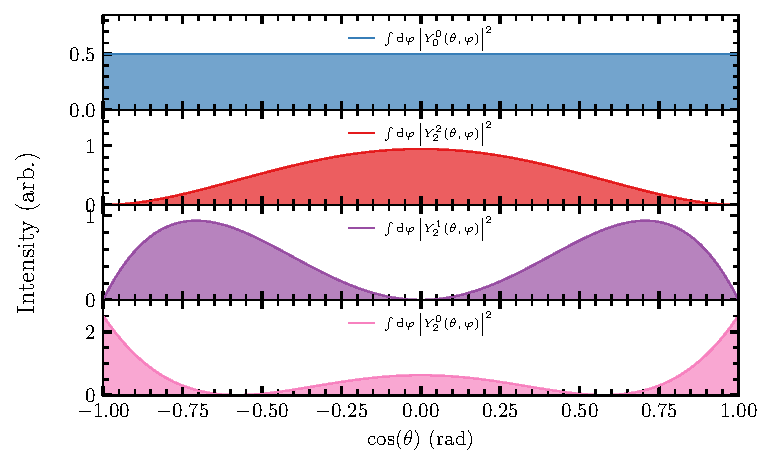
\includegraphics[width=.8\columnwidth]{spherical_harmonics}
  \label{fig:sph_harm}
  \caption{Absolute square of spherical harmonics for S- and D-waves integrated over $\varphi$.}
\end{figure}
% \begin{figure}[h]
%   \centering
%   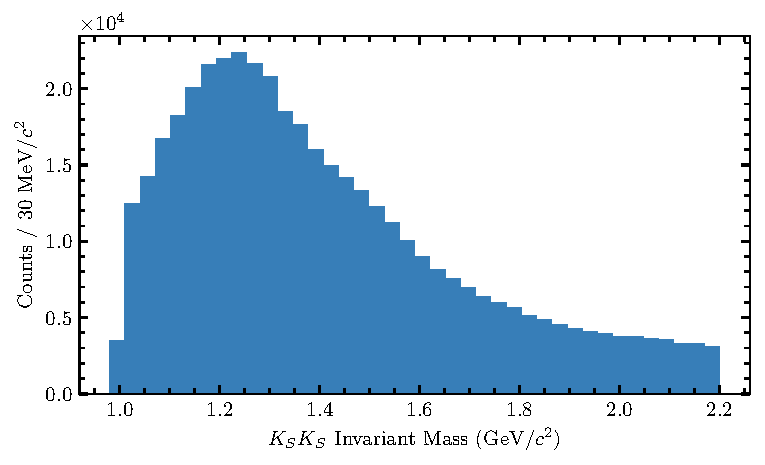
\includegraphics[width=.8\columnwidth]{KsKs_Inv_Mass_S17_fiducial}
%   \label{fig:mass_all_fiducial}
%   \caption{Absolute square of spherical harmonics for S- and D-waves integrated over $\varphi$.}
% \end{figure}


\subsection{Including Linear Polarization}
\section{The $Z_\ell^m$ Amplitude}
\section{The $K$-Matrix Parameterization}
\section{Waveset Selection}
